\chapter{General topology Partial Mesh Star}\label{chap:partial-mesh-star}
In this chapter will be described the process that led to the selection of the partial mesh star architecture, a model capable of applying the logical paradigms of edge/fog computing to a multi-cluster architecture while ensuring the possibility of deploying high-availability systems. Initially, the structural choices will be discussed, based on both the multi-cluster environment and the requirements of the adopted technologies (Percona, Liqo, etc.).

Potential use cases will then be described, demonstrating the flexibility of the logical hierarchical architectures that can be implemented. Finally, we will evaluate the characteristics and various limitations that this model entails.

\section{Cyber-Physical Architecture}
The first step was to consider how to abstract a logical model from the initial real-world situation. The electric power control and monitoring network, as shown in the Figure~\ref{fig:real-net}, can be schematized using both hierarchical tree topology graphs and peer-to-peer topology graphs.

\begin{figure}[ht]\centering
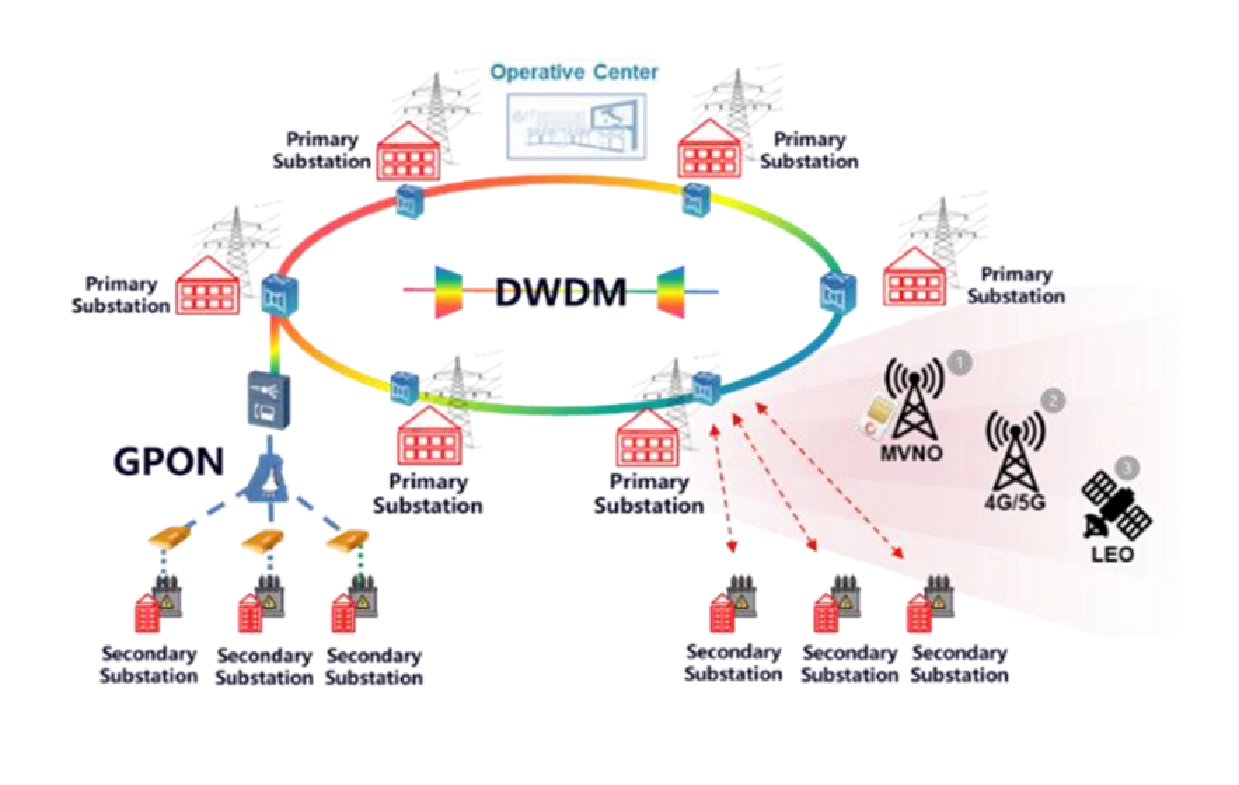
\includegraphics[scale=0.6]{Pictures/real-scheme-net}
\caption{Target Telecommunications Architecture Foreseen in the 2023 Development Plan for e-distribution.}\label{fig:real-net}
\end{figure}

Peer-to-peer should be discarded because, although the nodes representing the stations can be both data providers and receivers, the node representing the Area Control Center needs to exercise centralized control over all other nodes. Additionally, not all nodes have sufficient processing capabilities, especially if they represent secondary stations.

Among the various tree topology models, the star model is the only one that can be physically implemented using the standard version of Liqo. Indeed, it does not allow the offloading of an already offloaded namespace to prevent critical situations such as circular offloading. This means that all multi-level hierarchical topologies cannot be physically implemented without making customized changes to the technology's code. Moreover, distributed HA database systems tend to need to be in a single namespace, and multi-namespace solutions via operators do not support multi-cluster technologies as they cannot know the namespaces of other clusters.

The partial mesh version of the star model, which allows direct connections between leaves, is necessary for the correct transparent multi-cluster functioning of distributed database systems that rely on headless services. Each cluster that uses the same database system will need, in addition to having the offloaded namespace of the database, a direct connection with all other clusters, thus creating a partial mesh topology (partial because the connections do not necessarily have to be bidirectional).

\section{Logical hierarchy using labels and affinity}
A simple partial-mesh star topology offers only a two-level physical separation: a central node and the leaves. It lacks the necessary flexibility to manage the various real-world scenarios encountered in a monitoring and distribution network. Therefore, it is necessary to introduce a strategy to construct a complex logical topology on the existing physical model. This strategy is based on the use of Kubernetes' native label and affinity mechanisms.

Each cluster will be identified by a group of labels that specify its position in the desired logical topology and can be used by the scheduler to distribute the workload according to the intended logic. The node affinity mechanism can be used both to distinguish between different clusters and to differentiate the various nodes within a cluster, as it allows specifying different labels as targets. This way, one can define the label that identifies the cluster as well as the labels of the individual nodes within the cluster.

Pod affinity, on the other hand, is used to enforce coexistence conditions between pods on the same node. These mechanisms also offer a degree of flexibility, as they provide both "required" and "preferred" options. The "preferred" option allows the scheduler to prioritize the specified target for pod placement while still considering alternative targets if the preferred one is unavailable.

The following subsections will discuss some basic logical topologies, from which one can start to build their desired configuration.

\subsection{Independent Groups}\label{sec:indipendent-groups}
The leaf clusters of the partial-mesh star model are segmented into independent groups by assigning each node within the cluster a label that uniquely identifies its respective group. This method establishes distinct logical areas, as peering between clusters is only necessary within the same group (and only in case of using a distributed database system), to which separated workloads can be allocated. To enhance the delineation of these divisions, the root node could assign a separate namespace to each group, thereby also increasing security between them.

These groups are not mutually exclusive regarding the ownership of a node, provided there is no logical contradiction among the identifying labels. Consequently, a cluster may simultaneously belong to multiple groups, as demonstrated by leaf C in Figure \ref{fig:group-ind}.

\begin{figure}[ht]\centering
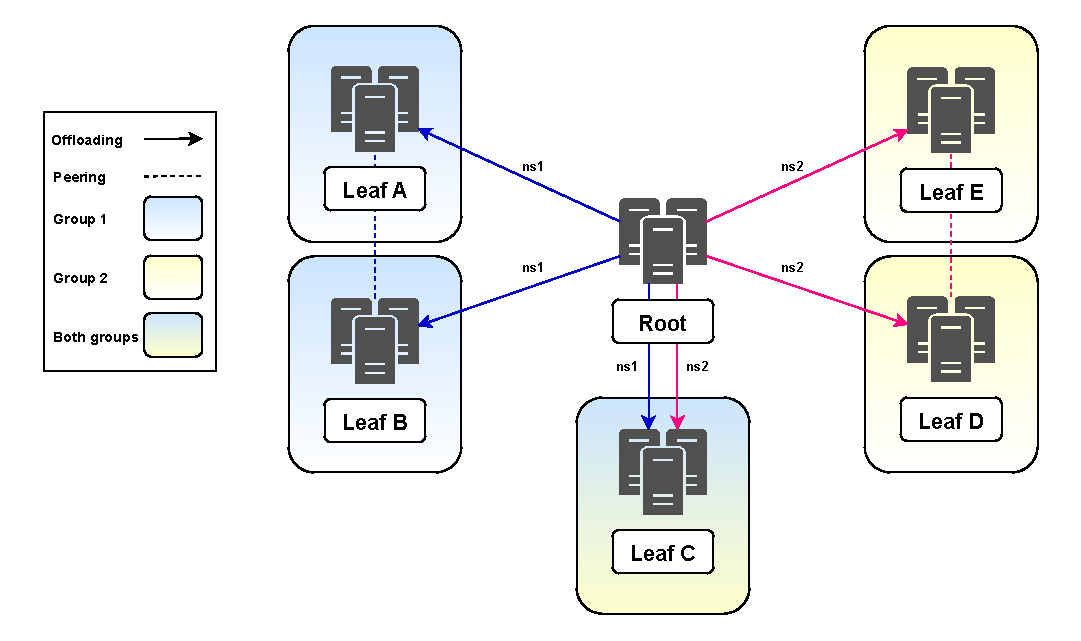
\includegraphics[scale=0.7]{Pictures/Group-v6}
\caption{Independent Groups Scheme.}\label{fig:group-ind}
\end{figure}

\subsection{Dependent Groups}
The leaf clusters of the partial-mesh star model are divided following a logical hierarchy by assigning a label indicating their position within the hierarchy. This approach creates dependent logical areas, as peering is necessary even between clusters belonging to different groups if a distributed database system is used. Figure~\ref{fig:group-dep} illustrates the worst-case scenario, where the database domain encompasses all leaf clusters. This topology supports new behaviors, such as allowing not only the selection of which groups to schedule workloads within the same domain.

This mechanism allows for the creation of multiple logical hierarchies within the same physical network, each with its own set of labels. Within a given logical hierarchical structure, a cluster can belong to only one group. However, when considering multiple structures, a cluster can belong to different groups.

\begin{figure}[ht]\centering
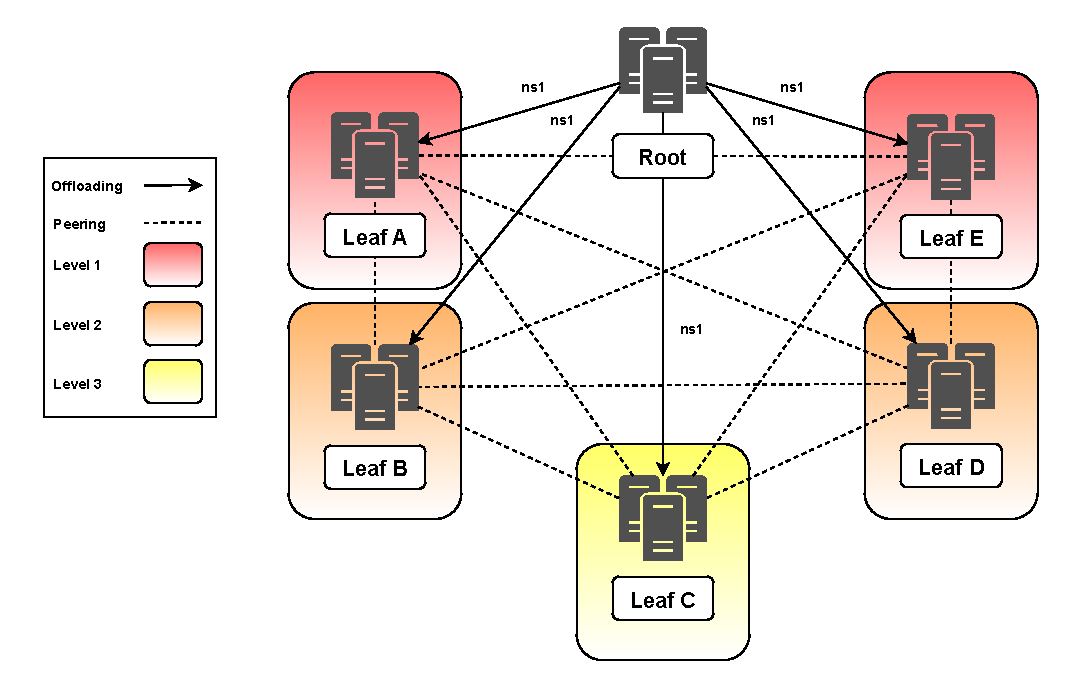
\includegraphics[scale=0.7]{Pictures/Level-v4}
\caption{Dependent Groups Scheme.}\label{fig:group-dep}
\end{figure}

\section{Partial Mesh Star Analysis}
As previously illustrated, the partial mesh star topology allows for the use of systems not originally designed for multi-cluster environments, such as distributed HA databases. However, this feature results in a quadratic increase in the number of peerings required between clusters within the database domain. This is because it requires at least a unidirectional peering full mesh. The number of links can be determined using the formula~\eqref{eq:eq-link-mesh}:
\begin{equation} \label{eq:eq-link-mesh}
\text{Link} = \frac{N(N-1)}{2}
\end{equation}
where N is the number of clusters.

The increase in the number of peerings only affects the time required to set up the entire architecture during its creation, as the consumption of additional resources is negligible, as noted in the article "Computing without Borders: The Way Towards Liquid Computing"~\cite{s2-1}.

The label mechanism offers substantial flexibility in selecting the logical architecture to overlay on the physical infrastructure. However, a drawback is the linear increase in setup time as the number of clusters expands. This characteristic renders the partial mesh star topology ideal for systems with relatively stable physical topologies, facilitating quick adjustments in logical configurations. While significant logical topological changes are supported, they require a corresponding setup time.

It should also be noted that this topology enhances the overall system resilience. Since clusters operate as independent entities, the architecture can support any number of disconnections as long as the central node remains unaffected. Therefore, resilience no longer depends on the number of disconnected clusters (as is the case in a Kubernetes cluster, where at least half plus one of the master nodes must remain healthy) but will instead depend on the constraints of the various applications installed within the architecture.
